	\documentclass[licencjacka]{pracamgr}
\usepackage[utf8]{inputenc}
\usepackage[T1]{fontenc}
\usepackage{amsmath}
\usepackage{amsthm}
\usepackage{graphicx}
\usepackage{wrapfig}
\usepackage{enumitem}
\usepackage{float}

\usepackage{listings}
\usepackage[english]{babel}

\usepackage[top=1in, bottom=1.25in, left=1.8in, right=1.8in,marginparsep=10pt,marginparwidth=100pt]{geometry} %usuncie te linijke, ona jest tylko po to by moje notatki na marginesach się miesciły
\usepackage[shadow,color=black!15,textsize=scriptsize]{todonotes}
\usepackage{xcolor}
\newcommand{\kdtodo}[1]{\todo[color=yellow!40,bordercolor=yellow,size=\footnotesize]{\textbf{TODO:}#1}}
\newcommand{\kdintodo}[1]{\todo[inline,color=yellow!40,bordercolor=yellow,size=\footnotesize]{\textbf{TODO:}#1}}
\newcommand{\krystynaintodo}[1]{\todo[inline,color=red!40,bordercolor=red,size=\footnotesize]{\textbf{TODO:}#1}}
\usepackage{hyperref}

\title{Inference in neural networks using low-precision arithmetic}
\author{Krystyna Gajczyk, Jakub Pierewoj,\\ Przemysław Przybyszewski, Adam Starak}
\nralbumu{332118, 360641, 332493, 361021}
\opiekun{Dr. Konrad Durnoga}
\kierunek{COMPUTER SCIENCE}
\klasyfikacja{  Computing methodologies - Machine learning - Machine learning approaches - Neural Networks}
\keywords{binarized neural network, XNORNET}
\dziedzina{ 11.3 Informatics, Computer Science}
\tytulang{Inferencja w sieciach neuronowych przy użyciu arytmetyki niskiej precyzji}
\begin{document}

\maketitle
\begin{abstract}
This project was created during "Team programming project" classes in 2016/17 and was proposed by Intel. We analyse some properties of binarized neural networks - the neural networks using binary parameter instead of floating-point numbers commonly used in deep learning. We experimented using different network structures and binarization algorithms to check accuracy and find ways to improve it.
\end{abstract}

\tableofcontents

\chapter{Introduction}
	
\section{What is deep learning and why is it interesting?}

Deep learning is a branch of machine learning which tries to model high level abstractions in data (like understanding words or finding objects on image) using a graph of simple elements - neurons, connected with specific activations and weights to others. It has recently gained a lot of interest from the industry, especially after recent successes in image or speech recognision.

The most important part of deep learning is training net based on the samples that the result is known. After each training step one can change weights and activation in model to make output of the network as close as possible to the expected value.

Currently deep neural networks get better results than state-of-the-art algorithms in many areas, such as computer vision and speech recognition. This breakthrough was possible because computing power of modern computers is high enough to handle intensive workload required to train large artificial neural networks.

\section{Why binarized networks are interesting?}
	Deep neural networks (DNN) usually use high precision (floating point) numbers to represent
	weights and activations. Computations using that arithmetic are usually handled by
	graphic cards. On devices with low computing power, such as mobile phones, use of deep neural networks is very limited.
	
	Researchers tried to address this problem in the number of papers in the recent years. A couple of main approaches have been investigated in order to reduce inefficient computation and memory usage in deep neural networks while maintaining the classification accuracy. Those approaches can be summarized as:

	\begin{itemize}
		\item Shallow networks - it has been proved, that every neural network can be replaced with a corresponding neural network with a single (possibly large) hidden layer. One of the main problems with this approach is, that in order to achieve similar accuracy as the original neural network, the shallow networks need approximately the same number of parameters (numbers of neurons and connection between them). Second problem is that empirical test have shown, that while it shows good results for relatively small datasets, it underperforms for larger datasets (such as ImageNet).
		\item Compression of pre-trained DNN - it is possible to prune a DNN at inference time by discarding the weights, that don’t bring any information to the classification process. It has been also further proposed to reduce the number of parameters and/or activations in order to increase acceleration, compression. This reduces the main blockers for using DNN on small, embedded devices, such as memory usage and energy. Memory usage can be achieved through quantizing and compressing weights with Huffman coding or hashing weights, such that the weights assigned to one hash bucket share the same parameter.
		\item Compact layers - this approach also reduces the memory usage and computation time. This approach replaces parts of the DNN structure with corresponding elements, which are smaller in size and bring nearly as much information. A few techniques have been examined, such as replacing a fully connected layer with global average pooling and replacing a convolution with a corresponding one requiring smaller amount of parameters.
		\item Quantizing parameters - this technique aims to replace the floating-point parameters of the neural network with the quantized values (through vector quantization methods), which require smaller number of bits of memory and need simpler arithmetic operations for computation. Number of DNN with quantization have been designed: 8-bit integer instead of 32-bit floating point activations, ternary weights and 3-bit activations instead of floating points, etc. It was shown, that this approach can lead to a DNN representation, which accuracy is not very far off from the state-of-the-art results.
		\item Network binarization - this is the extreme case of the parameter quantization technique. Due to a new learning algorithm, Expected Back Propagation, which bases on inferring network with binary weights and neurons through a variational Bayesian approach. Techniques using this approach mainly use the real-valued weights as a reference for their binarization. This idea was further extended to binarize both weights and activations, which was implemented in networks such as BinaryNet and XNOR-Net. 

	\end{itemize}

	Each DNN has its own tolerance of inference precision. There are numerous topologies of neural networks. Each topology indicates the number of layers and defines how the neurons are connected. The aim of this project is to study the structures and predict which one will behave the best in our environment. Dealing with 1-bit integer weights is going to strongly affect the complexity of computational algorithms and the size of data. The whole workflow is going to be much faster. 1-bit operations are way simpler than the 32-bit ones. Furthermore, the size of the inputs will require less memory. That is the perfect solution for less efficient devices. 
	\\\\
	Unfortunately, those properties will negatively affect the quality of prediction. Thus, the increase of the depth of chosen net should be also taken into consideration. A feature map is an input for the next level neurons.  The loss of data and weights precision can be alleviated by the increased number of the feature maps. We wanted to estimate ratio between number of feature maps in basic DNN and number of feature maps in low arithmetic precision DNN that maintain similar quality of the prediction.
	 To sum up, the research may bear out, that BDNNs have some great properties, which should be investigated much deeper. It may also find out, that they achieve better results in some cases and the present solutions should be replaced with BDNN.    

	\section{Our contribution}
	
	This project was created during "Team programming project" classes in 2016/17 and was proposed by Intel. Main goal of this project is the analysis of the effect that neural network binarization has on the inference quality of inference depending on:
	\begin{itemize}
	    \item network topology (LENET, ResNet, AlexNet)
	    \item level of binarization (weights or weights and inputs)
	\end{itemize}
	
	We have also tested if it is possible to achieve same accuracy as standard neural networks, which use floating point values, just by increasing the number of filters in convolutional layers.
	
	In addition to the main goal of this project, we have also added a binary convolution operation to TensorFlow.

\chapter{Dictionary}
    For reader's convenience, we have decided to include a dictionary containing some of the terms that we use in this paper. 
    
    \begin{itemize}
        \item Neural network - a machine learning model, inspired by the structure of a human brain. It consists of a large collection of neurons grouped into layers. Each neuron is connected to a set of other neurons. Each connection has an assigned value (also known as weight), which measures its importance.
        
        \item Inference (forward propagation) - a process of computing neural network's output based on its input and values of neuron weights.
        
        \item Backward propagation - a process of updating weights based on the difference between neural network output and the desired output.
        
         \item Activation - output of a single neuron.
        
        \item Training - repetitively performing inference and backward propagation until given stop condition (such as accuracy, number of iterations or lack of accuracy improvement) is met.
               
        \item Convolution - a mathematical function defined as follows: 
        $$ (f* g)(t) = \int_{-\infty}^{\infty} f(t)g(t-\tau)d\tau$$ where $$f,g: R\rightarrow R$$
        
        \item Convolution (discrete) - a mathematical function defined as follows: 
        $$ (f* g)(n) = \sum_{m=-\infty}^{\infty} f[m] g[n-m]$$ where $$f,g: Z\rightarrow Z$$
        
        \item Convolutional layer - a neural network layer which performs a discrete convolution operation between its inputs and weights (in this case they are usually called weight filters or kernels). Usage of this kind of layers proved to be successful in the field of image recognition, video recognition and natural language processing. 	
               
        \item Mini batch - a small subset of input data. It is usually a good practice to perform weight update after processing a mini batch instead of a single element of the training set.
        
        \item Batch normalization layer - a layer which returns a modification of its input such 
        that it has zero mean and unit variance.
        
        \item ReLU - a neuron activation function defined as follows: $$ R(x) = max(0,x) $$
        
        \item Epoch - one pass over all training set.
        
        \item Overfitting - effect which occurs when machine learning model fits to the noise of the training sample instead of the underlying trend behind the data. It has a negative effect on the neural network performance on the real data.
        
        \item Regularization - set of techniques which help to reduce overfitting.
        
        \item Dropout layer - a layer which returns a modification of its input such that some of the values are randomly set to zero. Dropout layers are used as a regularization technique.   
    \end{itemize}
\part{Architecture overview}
\chapter{Implemented binarization algorithms}
	\section{Binarized filters}

        In this approach we use special binarized filter for forward propagation.
        \\\\
        For an original filter $W$ forward propagation is:
        \begin{enumerate}
                \item Let $n$ be the number of elements in each filter, e.g. if filter is matrix $3 \times 3, n=9$.
                \item Let $W'$ be matrix containing signs of $W$.
                \item Calculate $A$ - average of elements for each filter in $W'$, so $A$ is a vector of size equal to number of filters in layer.
                \item Compute standard convolution using matrix $W'$.
                \item Return result of convolution multiplied by $A$.
        \end{enumerate}
        The back propagation is standard back-propagation made by using original W matrix. To achieve this result we override standard gradient to change sign to identity.
        \\\\
        In this type of binarizations, the gradients are in full precision, therefore the backward-pass still requires convolution between 1-bit numbers and 32-bit floating-points.

		\section{Binarized filters and activations}
		        For original filter W and input I forward propagation is:
		        \begin{enumerate}
		                \item Let n be the number of elements in each filter, e.g. if filter is matrix 3x3, n=9.
		                \item Let $W_{sign}$ be matrix containing signs of W divided by A.
		                \item Calculate A average of elements for each filter in $W_{sign}$, so A is a vector of size equal to numbers of filters in layer.
		                \item Let $I_{abs}$ be matrix with absolute value of input.
		                \item Let $I_{sign}$ be matrix with signs of input.
		                \item Let $K$ to be result of computation of standard convolution using as input $I_{abs}$ and as weights matrix containing $\frac{1}{n}$ on each position.
		                \item Compute standard convolution using input $I_{sign}$ and weights $W_{sign}$.
		                \item Return result multiplied by $K$ and $A$.
		        \end{enumerate}

	\chapter{Advantages of binarized neural network}
    One of the advantages of using binarized neural networks is that we can save trained weights as binary numbers and store them on a device with limited resources. What is more, it is also possible to optimize compute time. In this section, it is discussed exactly how much space and time we can save, when using different kinds of binarization.
    
    \section{Binarized weights}
        In this case we store binary value instead of a floating point for each weight. In addition, we also need to store coefficients $\alpha$ which are floating-point numbers. The amount of these coefficients depends on the type of binarization we perform. Computing $\alpha$ for each kernel compared to computing it for each layer gives us slightly worse space and computation time savings, but yields better accuracy.
        
        General formula for space savings is as follows (assuming we use 32 bit floating point numbers):
        $$s_m =  \frac{space_{bin}}{space_{float}} = \frac{\#_\alpha * 32bit + \#_{weights}*1bit}{\#_{weights} * 32bit} $$
        
        In case of different $\alpha$ for each layer $\#_\alpha = \#_{layers}$. So in in LENET, where $\#_{layers} = 4$ and $\#_{weights} = 1642272$ space saving coefficient $s_m = 1/(31.9975)$. If $\alpha$ is computed for each kernel, then $\#_\alpha = \#_{kernels}$. To compute the space savings for LENET model, we can observe that the number of weights is same as above, but $\#_\alpha = 32+32+1024+10 = 1098$, so $s_m = 1/(31.3297)$.
            
	    If we binarize weights, we can use the fact that to compute convolution we do not need to perform multiplication. This results in around 2x savings in compute time \cite{xornet}.
	    
	    \section{Binarized inputs and weights (XNORNET)}
	    Using this kind of binarization gives same savings as binarized weights, as we have to compute all $\beta$ coefficients during inference (they are not saved). Still, the space gain is around 32x which is an excellent result.
	    
	    In this case, it is possible to compute convolution using XNOR bitcount operations only. This results in around 58x savings in compute time \cite{xnornet}.

\chapter{Used networks and datasets}
		\section{LeNet on MNIST}
 		LeNet is a small 7-level network invented by Yann LeCun et al. It is one of the most known neural network due to it’s simplicity. Almost everyone, who is new to machine learning, begins with implementing it on MNIST dataset. However, it does not mean that LeNet is not a powerful tool. According to Wikipedia, couple of banks are applying LeNet to recognise written digits on cheques. Provided implementation was highly affected by Tensorflow's tutorial. \\
 		\subsection{MNIST}
 			MNIST is a subset of NIST. Each example represents a handwritten digit drawn in black\&white. Examples were resized and cropped, so that each digit is centered and the size is equal to $18\times18$ pixels. The dataset is split into 2 parts: training (60,000 pictures) and test (10,000 pictures).
 			\begin{figure}[h]
				\caption{Examples of MNIST pictures}
				\centering
				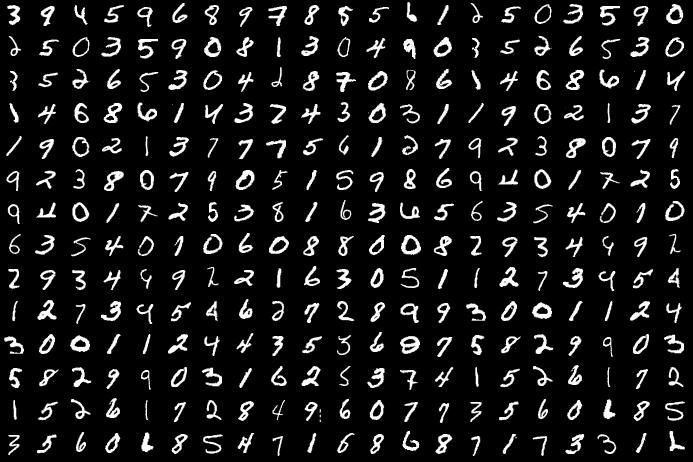
\includegraphics[width=\textwidth]{images/mnist}
			\end{figure}
 		\subsection{Network architecture}
 			\begin{itemize}
 			\item Convolution layer: kernel size $5 \times 5 \times 32$
 			\item Max Pool layer: kernel size $2 \times 2$
 			\item Convolution layer: kernel size $5 \times 5 \times 64$
 			\item Max Pool layer: kernel size $2 \times 2$
 			\item Fully-connected layer: $1024$ neurons
 			\item Dropout layer: $0.5$
 			\item Fully-connected layer: $10$ neurons
 			\end{itemize}
 			\begin{figure}[h]
				\caption{Scheme of LeNet}
				\centering
				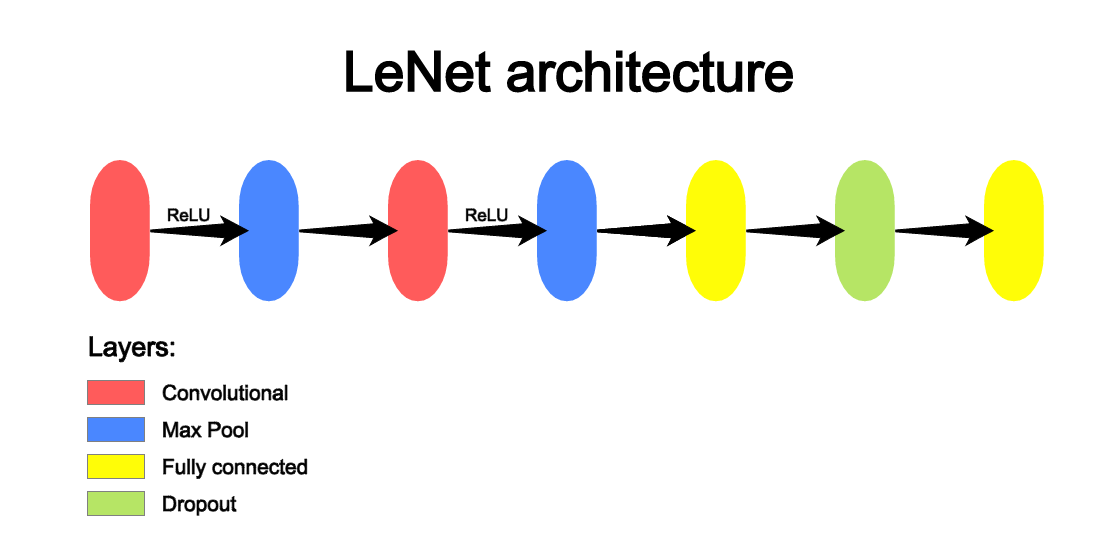
\includegraphics[width=\textwidth]{LeNet}
			\end{figure}
 		\subsection{Parameters}
 			\begin{itemize}
 			\item Weight initialization: truncated normal, stddev $0.1$
 			\item Optimizer: Adam Optimizer, learning rate $10^{-4}$
 			\item Error: softmax cross entropy with logits
 			\item Non-linearity: ReLU
 			\end{itemize}
 	\section{AlexNet on ImageNet}
 	AlexNet caused a huge breakthrough in deep neural networks after a great success during ImageNet Large-Scale Visual Recognition Challenge in 2012. It achieved top 5 test error rate of $15.4\%$ leaving other opponents far behind. In comparison, the next team achieved an error rate of $26.2\%$. 
 	\section{Finetuned AlexNet on oxford-102}
 	It has been 5 years since the astonishing victory of AlexNet, although people are still experimenting with it achieving great results. jimgoo(nick z gita, trzeba bedzie zacytowac) proposed a very clever approach of learning, which gave him a top 1 error rate of $7\%$ on oxford-102 set. In this experiment we try to replicate the results and find out whether it is possible to achieve similar accuracy using binarized network. 
 		\subsection{Oxford-flowers-102}
 			Oxford flowers dataset is containing the most common flowers found in United Kingdom. Each image represents a single flower. Within each class, the examples do not differ much, but there exists many similar classes, which makes the task harder. The images are saved in large scale and its’ sizes are not normalized. The dataset is split into 3 parts: test (6,149 pictures), train (1,020 images) and validation (1,020 images). In this experiment, the machine is trained on the test set and tested against the train set as the authors of CaffeNet fine-tuned on the Oxford 102 category flower dataset did.
 			\begin{figure}[h]
				\caption{Examples of Oxford-flowers-102 pictures}
				\centering
				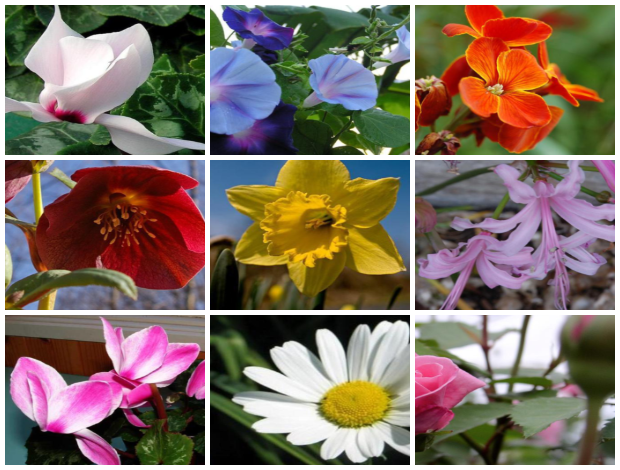
\includegraphics[width=\textwidth]{images/flowers}
			\end{figure}
 		\subsection{Network architecture}
 			\begin{itemize}
 			\item Convolution layer: kernel size $11 \times 11 \times 96$, learning rate $10^{-3}$
 			\item Max Pool layer: kernel size $3 \times 3$
 			\item Normalization layer
 			\item Convolution layer: kernel size $5 \times 5 \times 256$, learning rate $10^{-3}$
 			\item Max Pool layer: kernel size $3 \times 3$
 			\item Convolution layer: kernel size $3 \times 3 \times 384$, learning rate $10^{-3}$
 			\item Convolution layer: kernel size $3 \times 3 \times 384$, learning rate $10^{-3}$
 			\item Convolution layer: kernel size $3 \times 3 \times 256$, learning rate $10^{-3}$
 			\item Fully-connected layer: $4096$ neurons, learning rate $10^{-3}$
 			\item Dropout layer: $0.5$
 			\item Fully-connected layer: $102$ neurons, learning rate $10^{-2}$
 			\end{itemize}
 			\begin{figure}[h]
				\caption{Scheme of AlexNet}
				\centering
				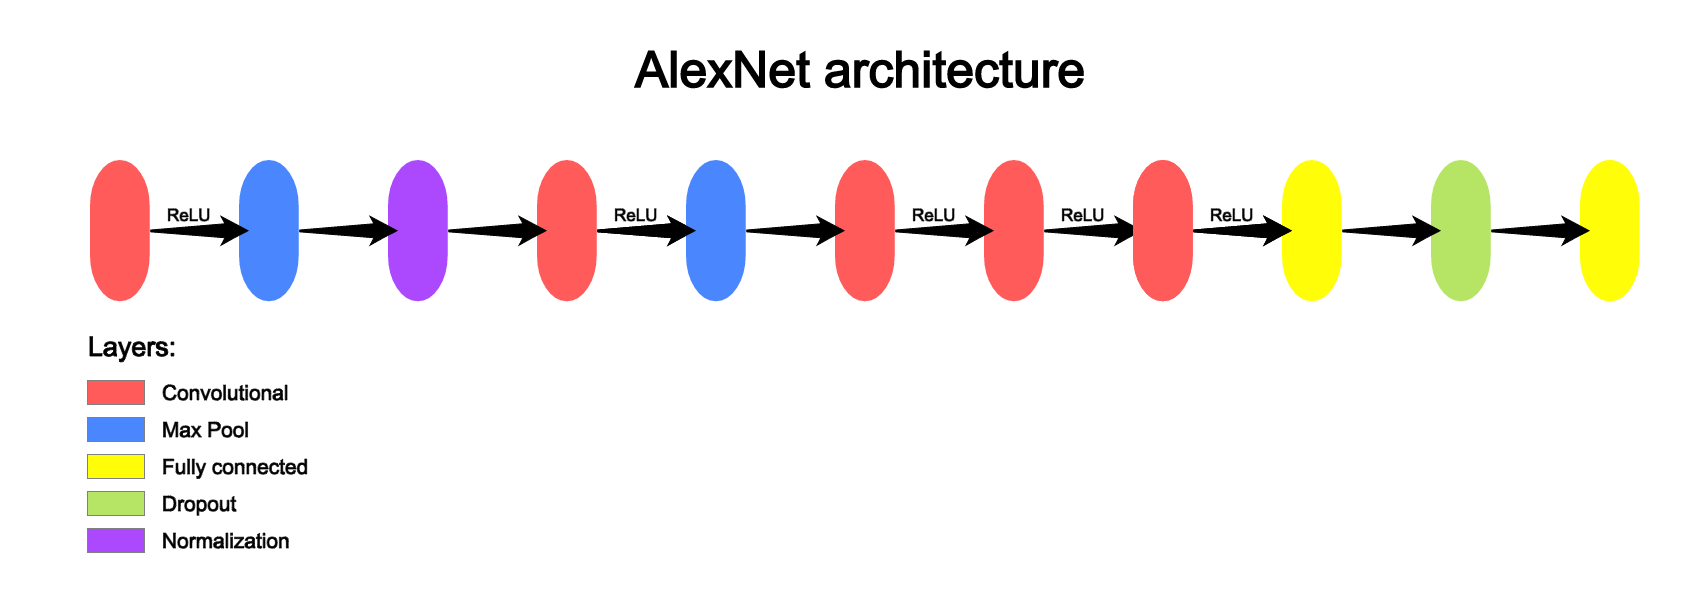
\includegraphics[width=\textwidth]{AlexNet}
			\end{figure}
 		\subsection{Parameters}
 			\begin{itemize}
 			\item Weight initialization: pretrained on ImageNet 2012 dataset
 			\item Optimizer: stochastic gradient descent
 			\item Error: softmax cross entropy with logits
 			\item Non-linearity: ReLU
			\end{itemize}
  	\section{Residual network on CIFAR-10}
		\subsection{CIFAR-10}
		CIFAR-10 is one of the most popular dataset. It is used for object recognition. It includes classes such as: airplanes, automobiles, birds, cats, deers, dogs, frogs, horses, ships and trucks. This dataset contains 60,000 images of size $32\times32$. Each class is represented by 6,000 images. The dataset was created by Alex Krizhevsky, Vinod Nair and Geoffrey Hinton. There also exists a bigger dataset called CIFAR-100.
		\begin{figure}[h]
				\caption{Examples of CIFAR-10 pictures}
				\centering
				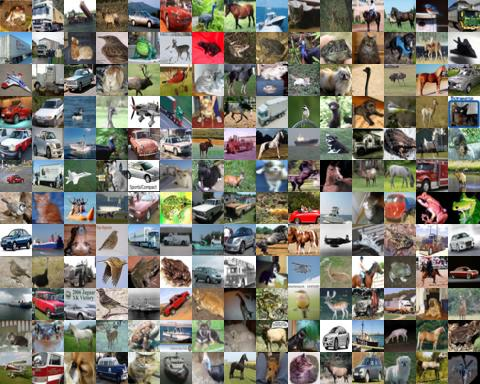
\includegraphics[width=\textwidth]{images/cifar-10}
			\end{figure}
		\subsection{Network architecture}
		Resnet is constructed using blocks. Every block($num\_filters$, $size\_filters$) contains:
		\begin{itemize}
			\item Normalization layer
			\item Convolution layer with $num\_filters$ of $size\_filters$ size
			\item Normalization layer
			\item Convolution layer with $num\_filters$ of $size\_filters$ size
			\item Identity connection which adds input to output of second convolution
		\end{itemize}
		\begin{figure}[h]
		\caption{TODO schemat bloku}
				\centering
				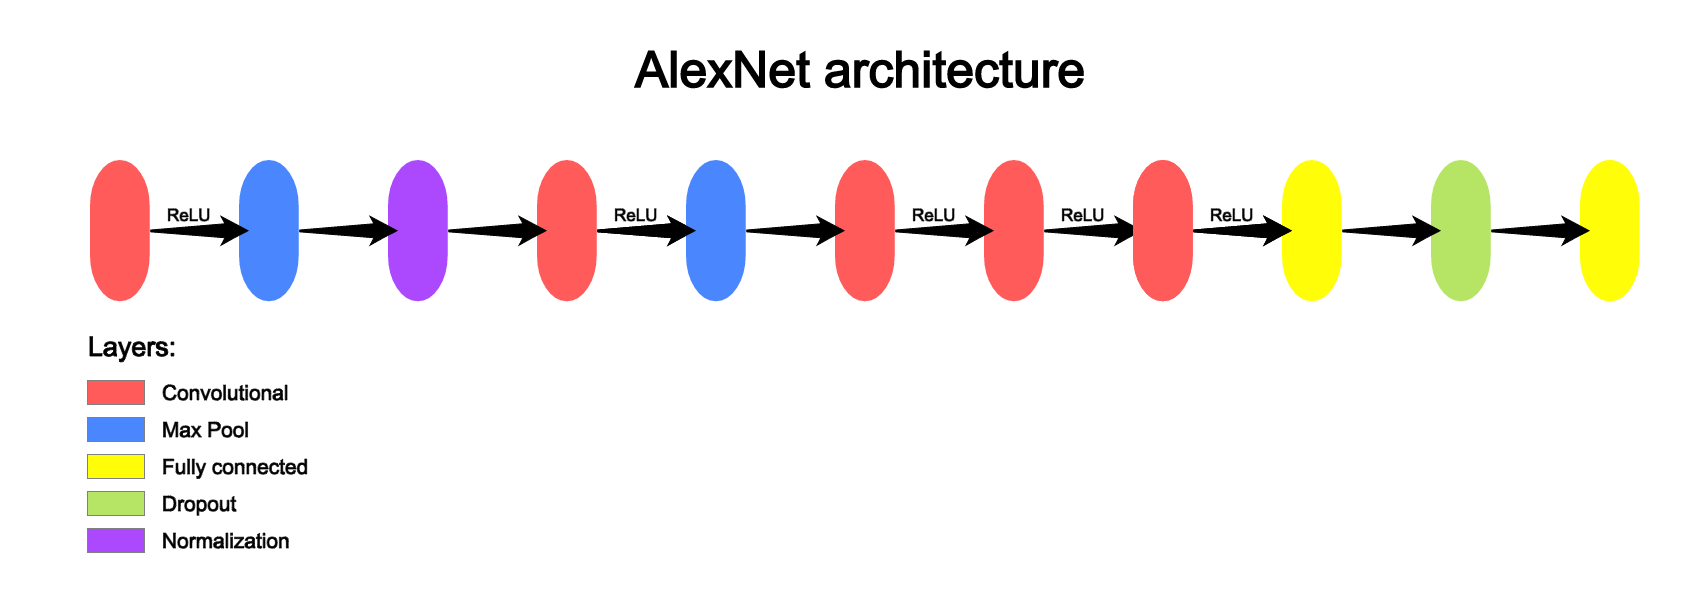
\includegraphics[width=\textwidth]{AlexNet}
		\end{figure}
		We use blocks to construct Resnet(n) in a following way:
		\begin{itemize}
			\item convolutional layer of size matching input of network (for CIFAR it is 32)
			\item n blocks(16,32)
			\item pool
			\item n blocks(32,16)
			\item pool
			\item n blocks(64,8)
			\item normalization 
			\item pool
		\end{itemize}
		\begin{figure}[h]
		\caption{TODO schemat resneta}
				\centering
				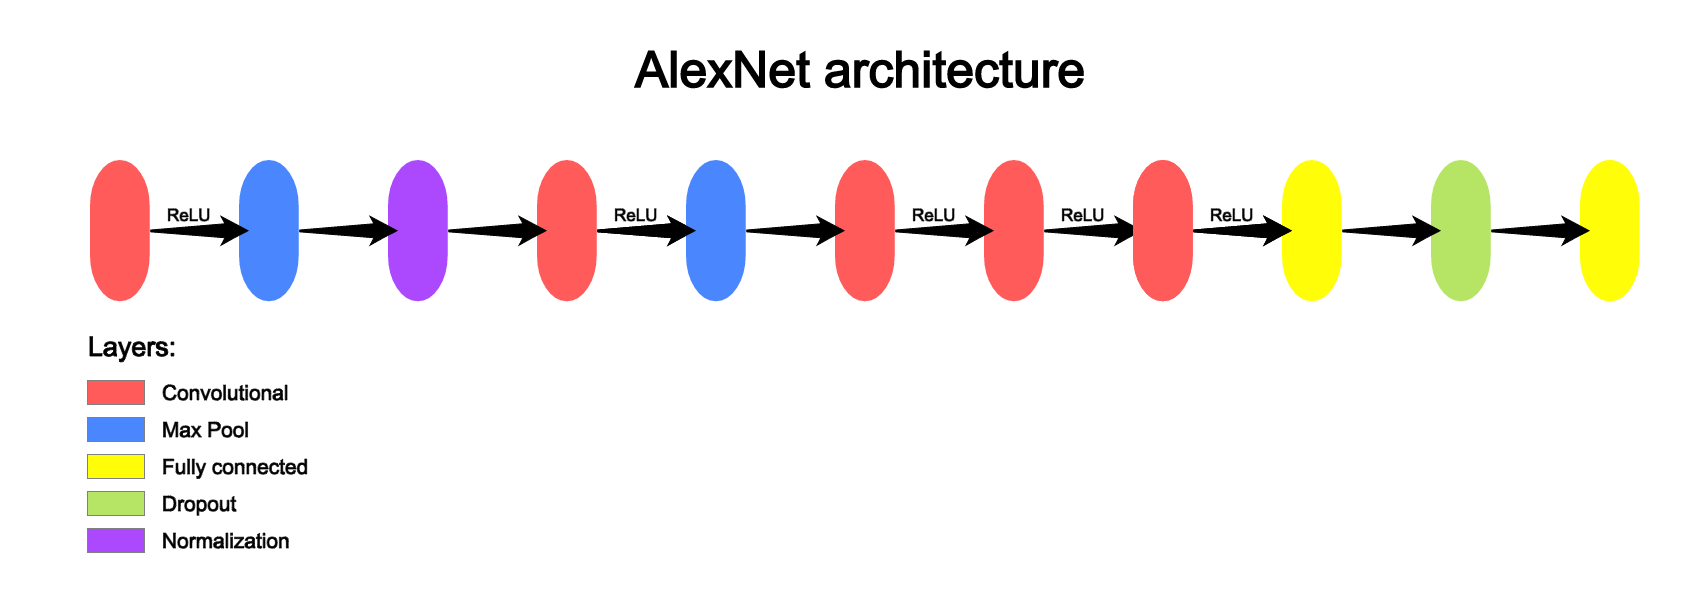
\includegraphics[width=\textwidth]{AlexNet}
		\end{figure}
		\subsection{Parameters}
			\begin{itemize}
 			\item Weight initialization: XAVIER initializer
 			\item Optimizer: momentum 
 			\item Error: softmax cross entropy with logits
 			\item Non-linearity: ReLU
			\end{itemize}

\chapter{The development process}

	\section{Used software tools}
	A range of external tools was used in order to organize work and to have a better overview of the current status of all of the ongoing tasks.
\\
	Git was chosen as a version control system for this project mainly due to its advantages when it comes to local branching and that every member of the team had some experience with this tool.
\\
	Our next tool was Jupyter notebook, which enabled us to write and share code more easily and made us more productive. 
\\
	When it comes to the build automation tool, there was no need to have one for the Python implementation and experiments. In case of the implemented C++ operation the team has used the build automation tool which is used by the Tensorflow framework, namely Bazel.	
\\
	To simplify communication between members of the team and other people involved in this project we used Slack, where a list of dedicated channels were created. This has helped in ordering the discussions over different topics, as one topic was hold in one channel.

	\section{Used methodology}

	The team worked in accordance with the Scrum Methodology with 1-week sprints. One of the members at the begining of the project was chosen to be the Scrum Master. Dividing workflow into separte tasks, which could be accomplished in a range of a week, helped with keeping the team updated with the project status. Also because of the weekly meeting every team member was updated about the work of the others. Due to the short length of the sprint it was easier for the team to prioritize work and adapt to the changes in our approach of delivering the requested software.
\\
	Our Scrum board was created in a tool called Trello. In this tool one can define the stages that each task has to visit when moving from the backlog to done. It is also easy to assign work to specific people and to add subtasks for bigger tickets. During the whole project the backlog was getting updated after the weekly meetings. At the top of the backlog the tasks of the highest priority were kept.

	\section{Used machine learning framework}

		We decided to work with one of the open source frameworks, that can be used for neural networks. The structure of BNN proposed in Binary Connect \cite{binaryConnect} and XNORNET \cite{xnornet} is very similar to the standard convolutional network, so there is no need to implement BNN from scratch. 
		\\
		All frameworks that we analyse (TensorFlow, Torch, Caffe) have similar functionality, for example they have already implemented pooling and affine layers so we can easily reuse them. 
\\
		From available frameworks we decided to choose TensorFlow \cite{tensorFlow}. It is an open source software library for numerical computation using data flow graphs. Nodes in the graph represent mathematical operations, while the graph edges represent the multidimensional data arrays (called tensors) transported between them. In case on of neural networks, nodes will represent layers of network. 
		The advantage of TensorFlow over other frameworks is really good community support and solid documentation.
\\		
		To perform our experiments more efficiently, we have used a higher level API for TensorFlow: TFLearn, which is a great tool for fast prototyping and creating proofs of concepts. It also provides great features for neural network visualization, such as weights plotting.

\chapter{Implementation details}

\section{Implementation in Python}
Tensorflow’s python library offers numerous built-in functions for machine learning and data exploring. Every operation is supplied with modifiable gradient. It significantly lessens the amount of effort and code written by the scientists. There are more advantages which stand for creating binary operations from included functions. First of all, almost every Tensorflow’s operation provides a GPU implementation. \\ It is a crucial feature. The computing power of GPU devices is much greater than CPUs one. Also, GPUs have an ability to perform more computations in parallel. Models trained on GPU are computed several times quicker due to parallelisation. Secondly, our binarized operations are less likely to have implementation bugs. Assuming that Tensorflow’s functions compute correctly, the only thing to do is compose them and modify the gradients so that it will fit XNORNET authors’ equations. It is a great advantage, especially on early stage, because future C++ operation can be based on it. \\ On the other hand, all the assets are lost. Tensorflow’s functions operate on float variables, each of which has 32bits. Additionally, it does not perform any xnor-counting operations. In fact, Python implementation of binarized convolution takes more time than the standard one. All the assets are only in the theory. Python’s binarized convolutions are created just for faster model computation. \\
		 
Tensorflow’s library provides a wrapper for a user-defined function. That is where it all started, but not for a long time. It quickly turned out that writing a custom function leads into trouble. The approach got changed. Instead of writing own function, we started to compose built-in ones. The most tricky part comes when parameters need to be binarized. \\ On the one hand, in feed-forward, the convolution must be computed with binary parameters. On the other hand, in backward propagation, the gradient must be computed with respect to the full-precision parameters. First part of this problem was solved by applying signum function. Unfortunately, this application affects the gradient computation. Changing the gradient function of signum to identity fixed the second part of the problem. (This fix was firstly applied in DoReFa-Net) The implementation supports both weights and weights \& inputs binarization. The second method does not compute redundant factors i.e. the second technique described in XNORNET paper is used.

		\section{Implementation in C++}
		It is possible in Tensorflow framework to add a so-called core user-defined operation to the already existing ones. To support binary convolution two operations were added, namely BinaryConv2D, which binarizes only filter weights, and BinaryConvInput2D binarizing both inputs and filters' weights. Those were implemented in source files conv\_bin.cc and conv\_bin\_inputs.cc respectively. Source files were added to the \/tensorflow\/core\/user\_ops directory.
\\\\
		First part of both kernel implenetations is validation of user provided data e.g. checking whether filter's and input's depth are equal and whether the strides attributes is well-defined.
\\\\
		Second part is where the calculation of binarized convolution is being conducted. Its design follows the algorithms described in section \ref{binarization_algorithm}. In both added operations a parameter 'alpha' is being calculated. The speed-up in its calculation was gained by using OpenMPI library and dividing the work of calculating summation of absolute values of filter's weights across all existing CPU cores.
\\\\
		In the BinaryConvInput2D kernel operation also calculation of parameter 'beta' is conducted. This required calculating averaged inputs accross channels and for each output's cell calculating an appropriate 'beta' parameter. Those parameters are being stored in a matrix 'K', which name was suggested in the referenced paper. Also in this case some speed-ups were implemented. In a naive implementation, calculation of matrix 'K' was doing repeated operations of calculating a sum over the same subset of input data. To avoid summing the same elements many times, a dynamic programming approach was used, in which the incremental sums are stored in a designated matrix 'D'.
\\\\	
		The last action is the binarized convolution. After binarizing the appropriate parts on data the resulting output of the convolution is multiplied by the corresponding 'alpha' and 'beta' parameters. Also in this case the operation was implemented in a way, that its calculation could be shared by all available CPU cores.
\\\\
		Both implementations follow a typical scheme of a Tensorflow operation. They consist of two sections - in one an operation is being declared (REGISTER\_OP) and in the second one the registered operation is being linked to the given kernel, that works on specific types and on a specific device (REGISTER\_KERNEL\_BUILDER). Our both implementations work only on CPU and on float types. 
\\\\
		A special build script was added, that was compiling our source files into a shared object file, which then was manually added in our Python tests and programs by a special Tensorflow call 'load\_op\_library'.
\\
		In order to test if the kernels computations are correct, unit tests were added to the library. Those tests are run every time the shared object file is being created.
	
	\chapter{Team members contribution}
	\section{Krystyna's contribution}
		\begin{itemize}
			\item organising the team's work (scrum master)
			\item contact with project supervisor
			\item implementation of Resnet
			\item experiments on Resnet
		\end{itemize}
	\section{Jakub's contribution}
		\begin{itemize}
			\item implementation of TensorFlow binarized convolution
			\item experiments on Lenet
			\item implementing C++ gradient for new operation
		\end{itemize}
	\section{Przemysław's contribution}
		\begin{itemize}
			\item contact with our partner company
			\item implementation of TensorFlow binarized convolution
			\item implementing qulity tests for project
		\end{itemize}
	\section{Adam's contribution}
		\begin{itemize}
			\item implementation of Alexnet
			\item experiments on Alexnet
			\item code review for collegues
		\end{itemize}

	
\part{Experiments results}
\chapter{Binarized vs standard network accuracy}

	\section{Lenet on MNIST}
		\subsection{Results and discussion}
		        \paragraph{Results} 
		     
		        The results of experiments are in table \ref{table:1}.
		        \begin{table}[H]
                    \caption{LeNet binarization on MNIST}
                    \centering
                    \begin{tabular}{c c c c c c}
                    \hline\hline
			    Full-precision & Binary weights & Binary weights \& inputs \\ [0.5ex]
                    \hline
			    98\% & 98\% & 95\% \\
                    \hline
                    \end{tabular}
                    \label{table:1}
	            \end{table}
	            \begin{figure}[h]
				\centering
				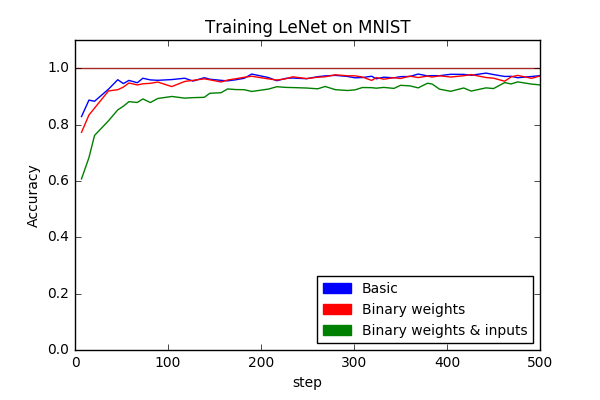
\includegraphics[width=\textwidth]{images/LeNet-training}
			\end{figure}
		        \paragraph{Discussion} 
			Both binarization methods acquired near state-of-the-art scores. The MNIST dataset is really simple and the LeNet structure is not complicated. Thus, the binarization does not significantly affect on the precision. The results are not surprising nor ground-braking. We made this experiment mostly for verifying our binarization methods.
	\section{AlexNet on Flowers}
		\subsection{Binarization results and discussion}
		        The results of experiments are in table \ref{table:1}.
		        \begin{table}[H]
				\caption{AlexNet on flowers-17 (50 epochs)}
                    \centering
                    \begin{tabular}{c c c c c c}
                    \hline\hline
			    Accuracy & Full-precision & Binary weights & Binary weights \& inputs \\ [0.5ex]
                    \hline
			    top-1 & 76\% & 79\% & 64\% \\
                    \hline
			    top-5 & 98\% & 95\% & 90\% \\
                    \hline
                    \end{tabular}
                    \label{table:1}
	            \end{table}
	            \begin{figure}[h]
				\centering
				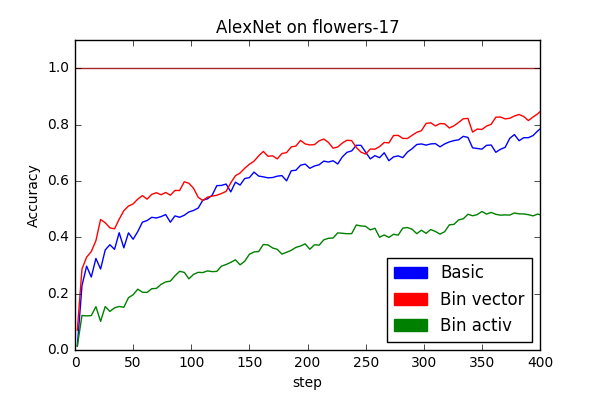
\includegraphics[width=\textwidth]{images/AlexNet-flowers17}
			\end{figure}
	            
		        \paragraph{Discussion} 
                        The results are promising considering the input images have high resolution. This experiment shows that fully binarized network does not lose as much precision as it was expected. Surprisingly, the binary weights network outperforms the full-precision one.
		\subsection{Fine-tuning results and discussion}
		     
		        The results of experiments are in table \ref{table:1}.
		        \begin{table}[H]
                    \caption{Fine-tuning AlexNet on flowers-102}
                    \centering
                    \begin{tabular}{c c c c c c}
                    \hline\hline
			    Full-precision & Binary weights vector factor & Binary weights scalar factor \\ [0.5ex]
                    \hline
			    85\% & 72\% & 63\% \\
                    \hline
                    \end{tabular}
                    \label{table:1}
	            \end{table}
	            \begin{figure}[h]
				\centering
				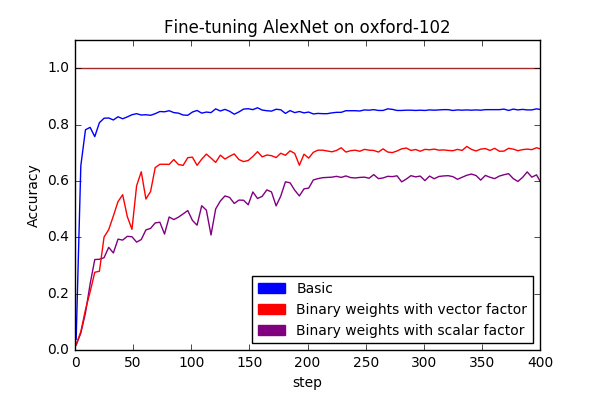
\includegraphics[width=\textwidth]{images/Fine-tuning-AlexNet}
		    \end{figure}
		        \paragraph{Discussion} 
			This experiment shows that binarized networks achieve near state-of-the-art performance also with pretrained weights, which were not trained on the binarized network.
	\section{Residual network on CIFAR-10}
		\subsection{Results and discussion}
			\subsubsection{Binary weights}
		        \paragraph{Results} 
		     
		        The results of experiments are in table \ref{table:1}.
		        \begin{table}[H]
                    \caption{Results of Resnet and BinResnet}
                    \centering
                    \begin{tabular}{c c c c c c}
                    \hline\hline
                    blocks & layers & learning rate & epochs & ResNet & BinResNet  \\ [0.5ex]
                    \hline
                            2 & 14  & 0.1   & 15 & 80\% & 77\% \\
                            5 & 32  & 0.1   & 15 & 82\% & 81\% \\
                            18& 110 & 0.1   & 20 & 84\% & 82\%\\
                    \hline
                            2 & 14  & 0.01  & 15 & 78\% & 76\% \\
                            5 & 32  & 0.01  & 15 & 79\% & 78\% \\
                            18 & 110 & 0.01 & 20 & 81\% & 80\% \\
                    \hline
                    \end{tabular}
                    \label{table:1}
	            \end{table}
	            \begin{figure}[h]
				\centering
				\caption{TODO: to jest fejkowy obrazek}
				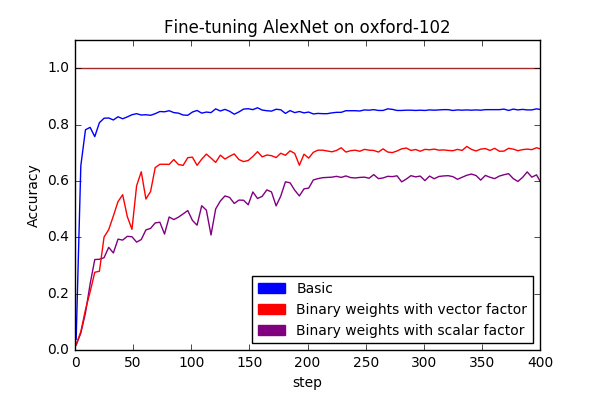
\includegraphics[width=\textwidth]{images/Fine-tuning-AlexNet}
			\end{figure}
		        \paragraph{Discussion} 

		        The results of binarized network are very good comparing to standard ResNet. The property of ResNet is preserved and the are no much difference in accuracy. That is very interesting result, because it shows that binarizing ResNet is only slightly decreasing accuracy so it is worth to use it to save memory and computation time, especially on CPU.

			\subsubsection{Binary Resnet with binary weights and inputs}
			        \paragraph{Discussion} 
				We did not manage to train any size of ResNet with binary weights and inputs, though the authors of XNORNET claim that their network achieves near state-of-the-art results. They did not provide any code, so we were struggling with it on our own. The size of the ResNet makes it very delicate. Small change in learning rate has a great impact on the accuracy. In this experiment, the greatest (still not satisfying) accuracy achieved ResNet-2 with score of 20\%. 
			        \begin{itemize}
			                \item Implementation which is using tf.nn.conv2d 2 times in each binarization process is much slower. 
			                \item Network with binarized both weights and activation is much harder to learn. In 2-layer Lenet the results were still very stable, but adding more layers, for example 14 in 2-blocks ResNet made network able to learn only during first few rounds of computation.
			                \item Smaller learning rate allows network to learn. Unfortunately the problem of deeper network still occurs, so the advantage of ResNet is not preserved.
			        \end{itemize}
\chapter{Increasing number of binarized filters}
	\section{LeNet on MNIST}
	\subsection{Discussion}
	Every binarization of LeNet achieved near stat-of-the-art results. The experiment in which we increase the amount of feature maps in LeNet has no value.
	\section{AlexNet on flowers-102}
	\subsection{Discussion}
	Combining pretrained feature maps with randomized one leads to trouble. Any network did not manage to converge. Only if the randomized parameters are set to values near 0, the networks start to learn. The problem is that new parameters do not have significant meaning, so this experiment reduces to the one in previous section. On the other hand, our resources are too small to obtain pretrained, scaled filters, because it requires to train AlexNet on ImageNet dataset, which has over 1.2 million of images.
	\section{AlexNet on flowers-17}
	\subsection{Discussion}
	Weights binarization led to the state-of-the-art performance, so we omit this case. Unfortunately, we did not manage to achieve greater performance on the binary weights \& inputs network with increased number of feature maps. The more we increased the amount of feature maps, the worse accuracy on testing set we achieved (3\% on average), though the training set accuracy rose (from 73\% to 80\%). It also requires about 3 times longer training.  We were not able to run networks with higher feature map ratio than 2, because the size of the network exceed the resources of our laptops.
	\section{ResNet on CIFAR-10}
		\subsection{Results}
		 The results of experiments are in table \ref{table:1}.
		\begin{figure}[h]
				\centering
				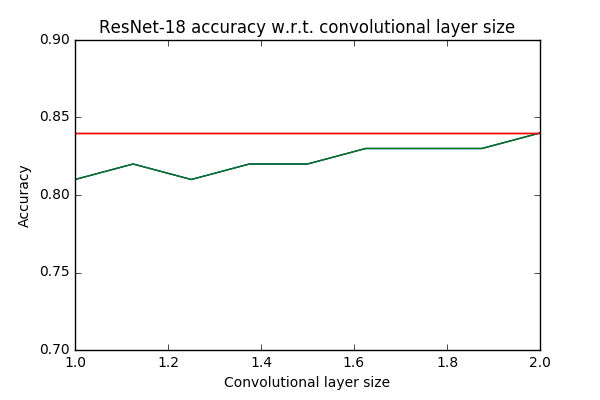
\includegraphics[width=\textwidth]{images/filter-ratio}
			\end{figure}
		\subsection{Discussion}
			Inscreasing number of filters is improving network accuaracy. When we give 2 times more filters in each convolutional layer we are getting accuracy of a non-binarized network.

\chapter{Conclusions}
	\section{Discussion of experiments results}
		Our experiments confirmed our expectation - binarized neural network can achieve accuracy which is very close to non-binarized networks. It works pretty well with simple architectures such as LeNet and AlexNet. On more complicated network, such as ResNet, there one must be very careful with setting up parameters. 
		\\\\
		For partially binarized network (with only filters binarized) we got great results for all tested architectures.
		\\\\
		For all networks increasing number of filters by around 100\% gave accuracy as good as the one of original network. This result is very promising - if we take twice much parameters, but each of them will be 32 smaller (after conversting float to bool) we still used 16 times less memory.

	\section{Future work}
		There are a couple of things, that could be further analyzed or added, namely:
		\begin{itemize}
			\item Right now only three ANN structures were tested. Those experiments could be extended to include also other popular structures such as GoogLeNet, VGG Net and ZF Net.
			\item Kernels in C++ are designed only for CPU. For potential speed-up gain new implementations of those operations on GPU could be added. 
			\item The current C++ implementation for binarizing both inputs and filter's weights is not saving any memory (it is using as much memory as the standard convolution operation). This could be improved by adding support for one or two bit types. 
			\item Right now it was only checked, how much the binarized network needs to be extended to achive the accuracy of its standard version. It could be also checked, what is the limit of achievable accuracy for the binarized networks and how many iterations are required to achieve the maximal accuracy on a given dataset.
		\end{itemize} 


\begin{thebibliography}{99}
\addcontentsline{toc}{chapter}{Bibliography}

\bibitem{understanding} Chiyuan Zhang, Samy Bengio, Moritz Hardt, Benjamin Recht, Oriol Vinyals, \textit{Understanding deep learning requires rethinking generalization}, https://arxiv.org/abs/1611.03530 (2016)

\bibitem{xnornet} Mohammad Rastegari, Vicente Ordonez, Joseph Redmon, Ali Farhadi, \textit{XNOR-Net: ImageNet Classification Using Binary Convolutional Neural Networks}, https://arxiv.org/abs/1603.05279 (2016)

\bibitem{binaryConnect} Matthieu Courbariaux, Yoshua Bengio, Jean-Pierre David, \textit{BinaryConnect: Training Deep Neural Networks with binary weights during propagations}, https://arxiv.org/abs/1511.00363 (2015)

\bibitem{resnet} Kaiming He, Xiangyu Zhang, Shaoqing Ren, Jian Sun, \textit{Deep Residual Learning for Image Recognition}, https://arxiv.org/abs/1512.03385 (2015)

\bibitem{tensorFlow} https://www.tensorflow.org/

\end{thebibliography}


\end{document}
